\documentclass[11pt]{article}

\usepackage[english]{babel}
\usepackage[margin=0.8in]{geometry}

% Math/Greek packages
\usepackage{amssymb,amsmath,amsthm, mathtools} 
\usepackage{algorithm, algorithmic}
\usepackage{upgreek, siunitx}
\usepackage{setspace}

% Graphics/Presentation packages
\usepackage{multirow}
\usepackage{graphicx}
\usepackage{cancel}
\usepackage{tabulary, enumitem, array}
\usepackage{xparse,mleftright,tikz}
\usepackage{physics}

% Misc packages
\usepackage{fancyhdr}


\usepackage[export]{adjustbox}

\usepackage{esint}

\sisetup{locale=US,group-separator = {,}}
\usepackage[colorlinks=true, allcolors=blue]{hyperref}


% Box function - update this as more sophisticated solutions are found
\newcommand\mybox[2][]{\tikz[overlay]\node[fill=blue!20,inner sep=2pt, anchor=text, rectangle, rounded corners=1mm,#1] {#2};\phantom{#2}}
\renewcommand{\arraystretch}{1.2}

% General macro declarations


\makeatletter
\let\oldabs\abs
\def\abs{\@ifstar{\oldabs}{\oldabs*}}
%
\let\oldnorm\norm
\def\norm{\@ifstar{\oldnorm}{\oldnorm*}}
\makeatother

\begin{document}

\title{PHSX 491: HW05}
\author{William Jardee}
\maketitle

\section*{Question 1}
\begin{enumerate}[label=\alph*)]
\item
\begin{align*}
\Delta \tau & = \int \sqrt{-\dd{s}^2} \\
& = \int \sqrt{-\left[-\left(1 - \frac{r_s}{R}\right)\dd{t}^2 + \left(1 - \frac{r_s}{R}\right)^{-1}\dd{r}^2 + R^2 \dd{\theta}^2 + R^2 \dd{\phi}^2\right]}\\
& = \sqrt{1 - \frac{r_s}{R}}\int \dd{t}\\
& = \left(1 - \frac{r_s}{R}\right)^{1/2} \, \Delta t
\end{align*}

\item At $R \rightarrow \infty$, the time goes to $1^{1/2} \, \Delta t = \Delta t$. As the radius get's larger and larger the time step get's closer to $1$. A.k.a. the closer to the event horizon, the slower the time, since the coefficient is always less than 1.

\item We are doing actual calculations, so we need to get some numbers to plug in. 
\begin{align*}
G & = 6.6704\times 10^{-11} \, \text{m}^2/\text{kg} \, \text{s}^2 & c & = 3.00\times 10^{8} \, \text{m/s}
\end{align*}
using this:
\[\Delta \tau = \sqrt{1 - \frac{2GM}{c^2 R}} \longrightarrow \qquad \Delta\tau(\alpha) \approx \sqrt{1 - \frac{1.48 \times 10^{-27}}{\alpha}}\Delta t\]
\[\boxed{\mqty{ \Delta\tau\left(\frac{5}{2}\right) & = \sqrt{1 - 1.93 \times 10^{-28}}\Delta t \vspace{0.5em}\\  \Delta\tau(3) & = \sqrt{1 - 4.94 \times 10^{-28}}\Delta t \vspace{0.5em} \\ \Delta\tau(6) & = \sqrt{1 - 2.47 \times 10^{-28}} \Delta t\vspace{0.5em} \\ \Delta\tau(100) & = \sqrt{1 - 1.48 \times 10^{-29}} \Delta t\vspace{0.5em} \\ \Delta\tau(1000) & = \sqrt{1 - 1.48 \times 10^{-30}}\Delta t}}\]
But, this is quite unwieldy. So, let's do this analysis by letting $G = c = 1$:
\[\boxed{\mqty{ \Delta\tau\left(\frac{5}{2}\right) & = 0.775\Delta t & = 0.775 \text{ hours}\vspace{0.5em}\\  \Delta\tau(3) & = 0.816\Delta t & = 0.816 \text{ hours}\vspace{0.5em} \\ \Delta\tau(6) & = 0.913 \Delta t & = 0.913 \text{ hours}\vspace{0.5em} \\ \Delta\tau(100) & = 0.995 \Delta t & = 0.995 \text{ hours}\vspace{0.5em} \\ \Delta\tau(1000) & = 0.999 \Delta t & = 0.999 \text{ hours}}}\]

\item 
So, time flows the slowest closer to $r_s$.

\item 
Inside the Schwarzchild radius the radical turns negative and thus we have an imaginary time. What does this mean? Isn't that a great question...
\item See Fig~\ref{fig:1.1}\\
My answers to the previous part doesn't change at all. In fact, graphing it was how I justified my answers to myself.
\begin{figure}[!ht]
\centering
	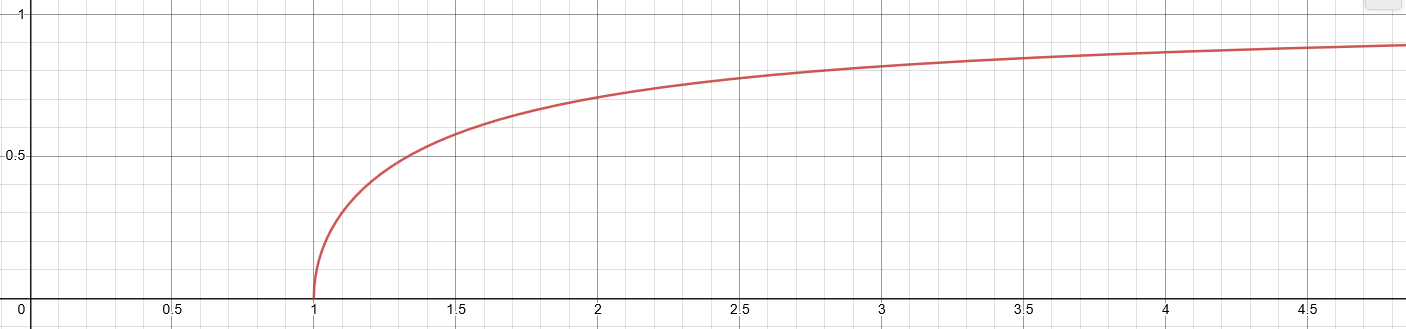
\includegraphics[width=0.9\textwidth]{phsx491_hw05_01.png}
	\caption{A qualitative graph of $g_{tt}$. Here $r_s = 1$, so the plot is effectively $\displaystyle \sqrt{1 - \frac{1}{x}}$.}
	\label{fig:1.1}
\end{figure}
\end{enumerate}

\end{document}
